%%%%%%%%%%%%%%%%%%%%%%%%%%%%%%%%%%%%%%%%%
% TMDEI Dissertation
% LaTeX Template
% Version 0.1 (Dec/2015)
%
% Adapted to TMDEI/ISEP style (Dec/2015) by
%  Nuno Pereira (nap@isep.ipp.pt) and
%  Paulo Baltarejo (pbs@isep.ipp.pt)
%
% Based on MastersDoctoralThesis Version 1.2 by Vel (vel@latextemplates.com) and
% Johannes Böttcher, downloaded from (21/11/15):
% http://www.LaTeXTemplates.com
%
% This template is originally based on a template by:
% Steve Gunn (http://users.ecs.soton.ac.uk/srg/softwaretools/document/templates/)
% Sunil Patel (http://www.sunilpatel.co.uk/thesis-template/)
%
% Template license:
% CC BY-NC-SA 3.0 (http://creativecommons.org/licenses/by-nc-sa/3.0/)
%
%%%%%%%%%%%%%%%%%%%%%%%%%%%%%%%%%%%%%%%%%

%----------------------------------------------------------------------------------------
%	PACKAGES AND OTHER DOCUMENT CONFIGURATIONS
%----------------------------------------------------------------------------------------

\documentclass[
11pt, % The default document font size, options: 10pt, 11pt, 12pt
%oneside, % Two side (alternating margins) for binding by default, uncomment to switch to one side (for drafting/reading purposes)
english, % english for English;
%portuguese,% for Portuguese; delete temporary files if you change language (e.g. 'make clean; make')
singlespacing, % Single line spacing, alternatives: onehalfspacing or doublespacing (for drafting/reading purposes)
%draft, % Uncomment to enable draft mode (no pictures, no links, overfull hboxes indicated)
%nolistspacing, % If the document is onehalfspacing or doublespacing, uncomment this to set spacing in lists to single
liststotoc, % Uncomment to add the list of figures/tables/etc to the table of contents (not recommended)
%toctotoc, % Uncomment to add the main table of contents to the table of contents (not recommended)
parskip, % Add space between paragraphs (recommended)
%nohyperref, % Uncomment to not load the hyperref package (not recommended)
nohyperreflinkcolor, % hyperref links are not colored (comment to color links, for example to produce an electronic-only version)
headsepline, % Uncomment to get a line under the header
]{tmdei-style} % The class file specifying the document structure

\usepackage{tikz} % Required for creating graphics programmatically (can be removed if not used)
%\usetikzlibrary{arrows} % Required for fancy arrows in TiKZ graphics (can be removed if not used)
\usepackage{multirow}
\usepackage{pgfplots} % Required for drawing high--quality function plots (can be removed if not used)
\pgfplotsset{compat=newest}

%
% Next you have examples of admissable citation styles; we recomend using the authoryear-comp citation style (which resembles Harvard); don't forget to only uncomment one
%

% authoryear-comp: recommended citation style (e.g. (Buendía, 1860), (Buendía 1910, Arcadio 1940))
%\usepackage[style=authoryear-comp,backend=biber]{biblatex} % Bibtex backend with the authoryear-comp citation style (authoryear citations, bibliography ordered alphabetically)

% numeric citation style (e.g. [1], [1-3])
\usepackage[style=numeric-comp,sorting=none,backend=biber]{biblatex} % Bibtex backend with the numeric-comp citation style (numeric citations, bibliography ordered by appearance)

% alphabetic citation style (e.g. [Buendía10], [Buendía10, Arcadio40])
%\usepackage[style=alphabetic,sorting=none,backend=biber]{biblatex} % Bibtex backend with the alphabetic citation style (alphabetic citations, bibliography ordered by appearance)


\addbibresource{mainbibliography.bib} % The filename of the bibliography

\makeglossaries % build the glossary

%----------------------------------------------------------------------------------------
%	THESIS INFORMATION
%----------------------------------------------------------------------------------------

\thesistitle{Explicação Automática de Conceitos} % Your thesis title, this is used in the title, print it elsewhere with \ttitle

%\thesissubtitle{{[}Thesis Subtitle{]}} % Your thesis title, this is used in the title, print it elsewhere with \tsubtitle

\author{André \textsc{Dias}} % Your name, this is used in the title page, print it elsewhere with \authorname

\subjectarea{Computer Systems} % Specialisation area (Computer Systems, Information and Knowledge Systems, Graphics, Systems and Multimedia, Software Engineering), used in the title page, print it elsewhere with \areaname

\supervisor{Dr. Nuno \textsc{Escudeiro}} % Your supervisor's name, this is used in the title page, print it elsewhere with \supname

%\cosupervisor{Dr. Jack \textsc{Smith}} % Your co-supervisor's name, this is used in the title page, print it elsewhere with \cosupname (comment, if no co-supervisor)

\committeepresident{Dr. Jonny Smith, Professor, DEI/ISEP} % Name of the president of the evaluation committee, print it elsewhere with \presidentname

\committeemembers{Dr. Jaimie Smith, Professor, DEI/ISEP\\Dr. Jones Smith, Professor, DEI/ISEP\\Dr. Jagger Smith, Professor, DEI/ISEP} % Name of the evaluation committee members (up to four), print it elsewhere with \committee

\keywords{Sign language, Text summarization, Automatic concept explanation} % Please define up to 6 keywords that better describe your work, print it elsewhere with \keywordnames

\university{\href{http://www.isep.ipp.pt}{Instituto Superior de Engenharia do Porto}} % Your university's name and URL, this is used in the title page and abstract, print it elsewhere with \univname

\department{\href{https://www.dei.isep.ipp.pt}{Departamento de Engenharia Informática}} % Your department's name and URL, this is used in the title page and abstract, print it elsewhere with \deptname

\thesisdate{Porto, \today} % thesis date,  print it elsewhere with \tdate

\hypersetup{pdftitle=\ttitle} % Set the PDF's title to your title
\hypersetup{pdfauthor=\authorname} % Set the PDF's author to your name
\hypersetup{pdfkeywords=\keywordnames} % Set the PDF's keywords to your keywords

\begin{document}

%----------------------------------------------------------------------------------------
%	FRONT MATTER
%----------------------------------------------------------------------------------------

% Include the frontmatter of your thesis here
% we include the glossary here (frontmatter is included with \input, so this command is as if it was in main.tex)
%All acronyms must be written in this file.
\newacronym{PSL}{PSL}{Portuguese Sign Language}
\newacronym{PL}{PL}{Portuguese Language}
\newacronym{API}{API}{Application Programming Interface}
\newacronym{MVP}{MVP}{Mininum Value Product}
\newacronym{DB}{DB}{Database}
\newacronym{NCD}{NCD}{New Concept Development Model}
\newacronym{CI}{CI}{Consistency Index}
\newacronym{CR}{CR}{Consistency Ratio}
\newacronym{RI}{RI}{Random Consistency Index}

\frontmatter % Use roman page numbering style (i, ii, iii, iv...) for the pre-content pages

\pagestyle{plain} % Default to the plain heading style until the thesis style is called for the body content

%----------------------------------------------------------------------------------------
%	TITLE PAGE
%----------------------------------------------------------------------------------------

\maketitlepage

%----------------------------------------------------------------------------------------
%	DEDICATION  (optional)
%----------------------------------------------------------------------------------------
%
%\dedicatory{For/Dedicated to/To my\ldots}
%\begin{dedicatory}

%\end{dedicatory}

%----------------------------------------------------------------------------------------
%	ABSTRACT PAGE
%----------------------------------------------------------------------------------------

\begin{abstract}
    Concept explanation has a great importance in languages with reduced lexicon that is not able to represent all the words of the Portuguese language.

    The users of LGP, when faced with words like 'Nanotechnology' have to resort to tools made for Portuguese because the ones available to them in LGP are not ideal.
    Those solutions, either lack translation features, which is the case of online dictionaries, or not practical, which is the case of sign language interpreters.

    To solve this problem, this project was created with the hypothesis of verifying if it's possible to utilize Text Mining, Information Scraping and Information Retrieval techniques to generate the explanation of a given word or expression that does not exist in the LGP lexicon.

    The planned solution consists in an Application Programming Interface (API) capable of generating an explanation of a given word or expression.
    This API will feed a web application responsible for receiving the user input and presenting the explanation in plain text and it's translation to LGP using an avatar.

    The solution is capable of displaying explanations in plain text, generated with the mentioned techniques, and exhibiting a clear indicator of their LGP readability for a deaf user.

\end{abstract}

\begin{abstractotherlanguage}
   A explicação de conceitos tem um papel importante em línguas com léxicos reduzidos, como é o caso das línguas gestuais.

    Em Portugal, a língua oficial utilizada pela comunidade surda, e as comunidades circundantes, tem o nome de Língua Gestual Portuguesa (LGP).
    Esta língua, como outras línguas gestuais, tem um léxico bastante reduzido o qual não é capaz de representar todas as palavras do Português.

    Os utilizadores da LGP, quando são confrontados com palavras como Nanotecnologia têm de recorrer a ferramentas criadas para Português, uma vez que as ferramentas disponíveis para LGP não uma solução ideal.
    Estas soluções, ou apresentam falhas na funcionalidades de tradução, que é o caso dos dicionários online, ou não são praticas, como é o caso dos intérpretes de língua gestual.

    Para dar resposta a este problema, este projecto foi criado com a hipótese de verificar se é possível utilizar técnicas de \textit{Text Mining}, \textit{Information Retrieval} e \textit{Information Scraping}, para gerar a explicação de uma palavra ou expressão que não faça parte do léxico da LGP.

    A solução proposta consiste numa \textit{Application Programming Interface} (API) que é capaz de gerar a explicação de uma dada palavra ou expressão.
    Esta API irá comunicar com uma aplicação web que é responsável por receber os \textit{inputs} do utilizador e apresentar as explicações geradas em texto, assim como a tradução para LGP utilizando um avatar.

    A solução final é capaz de apresentar, em texto, as explicações geradas utilizando as técnicas mencionadas assim como exibir de forma clara, ao utilizador surdo, o indicador de legibilidade de LGP associado a cada explicação.

\end{abstractotherlanguage}

%----------------------------------------------------------------------------------------
%	ACKNOWLEDGEMENTS (optional)
%----------------------------------------------------------------------------------------

\begin{acknowledgements}
    Firstly, to Instituto Superior de Engenharia do Porto for all the knowledge it allowed me to get and all the support it's teachers provided, with special focus on Dr. Nuno Escudeiro for being my supervisor in this project.

    To my best friend Tiago Soares, for all the support, advice and company, through all the happiness and sadness.Words will never be enough to repay your friendship.
    Also for following your dreams and taking the academic path I'm now here finishing. Always remember, "May we get what we want, may we get what we need, but never what we deserve".

    To my friend Miguel Carneiro, for all the knowledge, help, good conversations and for the motivation to always seek to improve myself.

    To my friends Carlos Figueiredo, Diogo Monteiro, Pedro Rodrigues and João Guedes, for all the moments we shared during the praxis and late night gatherings.

    Finally, and most importantly, to my parents Artur Dias and Maria Fernanda Dias, for all the sacrifices they made so I was able to have a safe and healthy home, even in dire times.
    This allowed me to have the time and space to pursue a higher education, which was an opportunity they never had.

    To all of you, my deepest and most sincere thank you,

    André Dias

\end{acknowledgements}

%----------------------------------------------------------------------------------------
%	LIST OF CONTENTS/FIGURES/TABLES PAGES
%----------------------------------------------------------------------------------------

\tableofcontents % Prints the main table of contents

\listoffigures % Prints the list of figures

\listoftables % Prints the list of tables

%\iflanguage{portuguese}{
%\renewcommand{\listalgorithmname}{Lista de Algor\'itmos}
%}
%\listofalgorithms % Prints the list of algorithms
%\addchaptertocentry{\listalgorithmname}


\renewcommand{\lstlistlistingname}{List of Source Code}
\iflanguage{portuguese}{
\renewcommand{\lstlistlistingname}{Lista de C\'odigo}
}
\lstlistoflistings % Prints the list of listings (programming language source code)
\addchaptertocentry{\lstlistlistingname}


%----------------------------------------------------------------------------------------
%	ABBREVIATIONS
%----------------------------------------------------------------------------------------
%\begin{abbreviations}{ll} % Include a list of abbreviations (a table of two columns)
%%\textbf{LAH} & \textbf{L}ist \textbf{A}bbreviations \textbf{H}ere\\
%%\textbf{WSF} & \textbf{W}hat (it) \textbf{S}tands \textbf{F}or\\
%\end{abbreviations}

%----------------------------------------------------------------------------------------
%	SYMBOLS
%----------------------------------------------------------------------------------------

%\begin{symbols}{lll} % Include a list of Symbols (a three column table)

%$a$ & distance & \si{\meter} \\
%$P$ & power & \si{\watt} (\si{\joule\per\second}) \\

%%Symbol & Name & Unit \\

%\addlinespace % Gap to separate the Roman symbols from the Greek

%$\omega$ & angular frequency & \si{\radian} \\

%\end{symbols}



%----------------------------------------------------------------------------------------
%	ACRONYMS
%----------------------------------------------------------------------------------------

\newcommand{\listacronymname}{List of Acronyms}
\iflanguage{portuguese}{
\renewcommand{\listacronymname}{Lista de Acr\'onimos}
}

%Use GLS
\glsresetall
\printglossary[title=\listacronymname,type=\acronymtype,style=long]

%----------------------------------------------------------------------------------------
%	DONE
%----------------------------------------------------------------------------------------

\mainmatter % Begin numeric (1,2,3...) page numbering
\pagestyle{thesis} % Return the page headers back to the "thesis" style


%----------------------------------------------------------------------------------------
%	MAIN BODY
%----------------------------------------------------------------------------------------

% Include the chapters of the thesis as separate folder for each chapter
% Uncomment the lines as you write the chapters

% Chapter 1
% 
\chapter{Introduction} % Main chapter title
\label{chap:Chapter1} % For referencing the chapter elsewhere, use Chapter~\ref{Chapter1}

The aim of this chapter is to present the developed work.
It is possible to find the project's problem and its context, followed by the objectives defined to create a possible solution.

\section{Context}

Learning is the act or process of acquiring knowledge, and it's a part of the human life from birth to death.
This ability is shared by humans and animals and it's being partially implemented to machines with the help of machine learning.
Humans learn by interaction with other others or the environment.

The traditional way of learing is known as rote learning and it is defined by the memorization of information based in repetition.
It has the advantage of quickly developing basic knowledge, an example of this is teaching a kid the alphabet or the numbers.
A major disadvantage of this approach is not be able to be used to teach more complex or abstract subjects or subjects that can have different meaning based on context.
Explaning a thopic like "Love" is not possible with this methodology.

One alternative to rote learning is meaningful learning, also known as conceptual learning.
Meaningful learning focus on understanding new knowledge and how it is related to the previously obtained.
One disadvantage of this approach is that not every human has the same previous knowledge, therefore, if not tailored, it wil take different people different time to be understand. 
On the other hand, a major advantage is the encouragement of understanding which benefits retention of knowledge.

Novak (\citeyear{novak_2012}) wrote in is book that meaningful learning has three requirements : 

\begin{itemize}
    \item Relevant prior knowledge - The learner must already process information that has some relation to the new information to be learned.
    \item Meaningful material - It is composed by significant concepts and relevant to other, already acquired, knowledge.
    \item The willing to learn meaningfully - The learner chooses to consciously relate new knowledge to relevant knowledge already obtained.
\end{itemize}

Concepts are the key aspect of this approach, that help humans understand and realate knowledge.
Concepts are abstract or generic ideas that have a common set of features that are shared across multiple situations and contexts.

Humans have learned concepts even if they are not aware of it.
An example of it is shown everytime they take a sit on chair.
Chairs can take very different designs but they all share some characteristic, such as having a mean of support, a seat and a back rest.
The concept of chair is made by those shared characteristic and once one understandes that concept he will be able to identify most chairs as such.

\section{Problem}

Concept explanation can take a fundamental part of the learning process, whether it takes place in an educational environment, a day-to-day or a profissional context.
The importance of concept explanation is even greater when it comes to languages with a small lexicon, in particular sign languages.

According to the World Health Organization (\citeyear{who_2018}), as of march 2018, there were 466 million people with desabling hearing loss, this represents 5\% of the world population.
Without being able to hear, deaf people are not able to communicate using sound therefor they must use sign languages.

The number of different sign languages are not precisely defined, but most countries have their one sign language.

In Portugal the language used by the deaf community is known as \gls{PSL}.
The lexicon of \gls{PSL} is composed by multiple signs where each once represents a word or an expression of the \gls{PL}.
However, there are numerous words in \gls{PL} that don't have a sign that translates them.
Those words/expressions have to be explained using the available lexicon.

This problem is recurrent when it comes to scientific domains.
One example of this, is the a concept like 'Nanotechnology' which doesn't have a sign for it, and so it's necessary to explain it using other words.

\section{Objectives}

Taking into consideration the problem previously explained, the first goal is to develop an \gls{API} that is capable of generating the explanation of a given word or expression.
To be able to produce said explanation the \gls{API} will use Text Mining, Information Scraping and Information Retrival techniques.

The developed \gls{API} will be used to create a web application, that presents the user with an explanation for the input given.
To present the explanation the application will use text, as well as an avatar that will convert said text to \gls{PSL}.
The avatar was developed in another GILT project, and is already in use in another web application also related to \gls{PSL}.

Future or already existing projects made by GILT may use this \gls{API} to further enchance their functionalities.

This project has the intent to make it easier to produce content in \gls{PSL}, and by doing so, promoting the inclusion and equality of opportunities for the deaf community. 

% Chapter 2

\chapter{Context and the State of Art}
\label{chap:Chapter2}

This chapter presents a review of the most relevant topics (e.g. Information Retrival, Information Extraction) and similar approaches to the problem to be solved.

\section{Information Retrival}

\dots

As the name suggests, Information Retrival, is the act of retriving information from a source.
But this definition can be very broad.
Christopher D. Manning et al. (\citeyear{Reference4}) wrote on his book that Information Retrival is finding materials of an unstructured nature that satisfies an information need from within large collections.

\section{Information Extraction}

\dots

\section{Related Work}

The goal is to investigate approaches to the problem of generating a definition, or explanation to a given word or expression.


% Chapter 3

\chapter{Value Analysis} % Main chapter title
\label{chap:Chapter3} % For referencing the chapter elsewhere, use \ref{chap:Chapter3}

In order to develop a new product there is a need for a value analyzing in order to properly assess the relation between cost and value.
This analysis is presented in the following subsections.

\section{New Concept Development Model}

The \gls{NCD}\cite{koen2001providing} is a methodology that supplies a structure to transform an opportunity in a concept by following its key stages.
This will help understand the opportunity value in a well defined manner.

The five key stages, that compose the model defined by Koen\cite{koen2001providing}, were used to define the opportunity behind this project.

\begin{itemize}
    \item \textbf{Opportunity identification} - The opportunity was identified by a member of the deaf community.
    He claimed that there were no solutions to help the process of explaining a given concept using sign language.
    The lexicon of \gls{LGP} is quite small so most words don't have a direct translation, therefore it is required to use the available gestures to explain them.

    \item \textbf{Opportunity analysis} - When analyzing the market, the only tools that have some similarities are the sign language dictionaries but they have some limitations that make it impossible to be a viable solution.
    One of these limitations is that a translation to be added requires that a person is recorded performing the signs required to reproduce the word or expression.
    Another limitation of those dictionaries is the lack of translations for word from the scientific domain.

    \item \textbf{Idea creation} - In this stage, some ideas were formulated for a solution that targets the identified opportunity and is a better fit over the other alternatives analyzed.
    One idea is that the solution to be developed makes the process of explaining a concept automatic.
    For this, the explanation can be found somewhere online and it is possible to obtain it using information retrieval, information extraction and text mining techniques.
    To make the obtained explanation viable to be presented to a member of the deaf community it would be better to translate it to \gls{LGP}.
    For this, there is another GILT project that is already capable of performing this translation and the \gls{API} behind it can be used in this solution.

    \item \textbf{Idea selection} - In this stage, the goal was to take all the possible ideas and approaches into a single one that fulfills the necessary requirements.
    The resulting idea is to develop an automatic interpretation system having the needs of the deaf community in mind.
    This system will use Information retrieval, information extraction and text mining to generate the explanation of a given word or expression.
    It will also translate said explanation to \gls{LGP}.

    \item \textbf{Concept definition} - After having the idea selected, the next step is to define the objectives needed to achieve it.
    The goals of this project are to develop an \gls{API} capable of generating the explanation of a given concept and a web application that will use this, and another \gls{API} to help the deaf community in the process of concept explanation.

\end{itemize}

\section{Value}

The perceived value is based on the benefits and sacrifices identified.

\begin{table}[H]
\caption{Perceived Value}
\label{tab:pValue}
\centering
\begin{tabular}{|m{3cm}|m{3cm}|m{3cm}|m{3cm}|}
\hline
\tabhead{} & \tabhead{Product} & \tabhead{Service} & \tabhead{Relationship} \\
\hline
Benefit & Knowledge & Utility & Trust\\
\hline
Sacrifice &  & Search costs & \\
\hline
\end{tabular}
\end{table}

\section{Value Proposition}

With the goal of helping the process of concept explanation, with focus on the inclusion of the deaf community, this solution aims to use information retrieval, information extraction and text mining techniques to develop a system capable of generating an explanation of a given word or expression and also provide the \gls{LGP} translation.

\section{Business Model Canvas}

In order to ensure a solid structuring of the various business characteristics, it's necessary to use tools that help in the strategic management planning.
The tools to be used must help answer some question, such as:

\begin{itemize}
        \item Who are the clients?
        \item What do they value?
        \item How can we reach them?
        \item What skills are required?
        \item What are the costs associated with our solution?
\end{itemize}

One of the tools that is able to help in this is the Business Model Canvas\cite{osterwalder2010business}, that provides 9 key blocks to aid in the process of planning the business concepts.
The 9 key blocks are:

\begin{itemize}
    \item \textbf{Key Partners} - Describes the network of suppliers and partners that make the business model work.
    \item \textbf{Key Activities} - Describes the most important things a company must do to make the business model work.
    \item \textbf{Key Resources} - Describes the most important assets required to make a business model work.
    \item \textbf{Value Propositions} - Describes the bundle of products and services that create value for the Customer Segments.
    \item \textbf{Customer Relationships} - Describes the types of relationships a company establishes with the Customer Segments.
    \item \textbf{Channels} - Describes how a company communicates with and reaches its Customer Segments to deliver a Value Proposition.
    \item \textbf{Customer Segments} - Defines the different groups of people or organizations a company aims to reach and serve.
    \item \textbf{Cost Structure} - Describes all costs incurred to operate a business model.
    \item \textbf{Revenue Streams} - Represents the money a company generates from each Customer Segment.
\end{itemize}

In Figure~\ref{fig:CANVAS} it is illustrated the Business Model Canvas created for this project.

\begin{figure}[H]
\centering
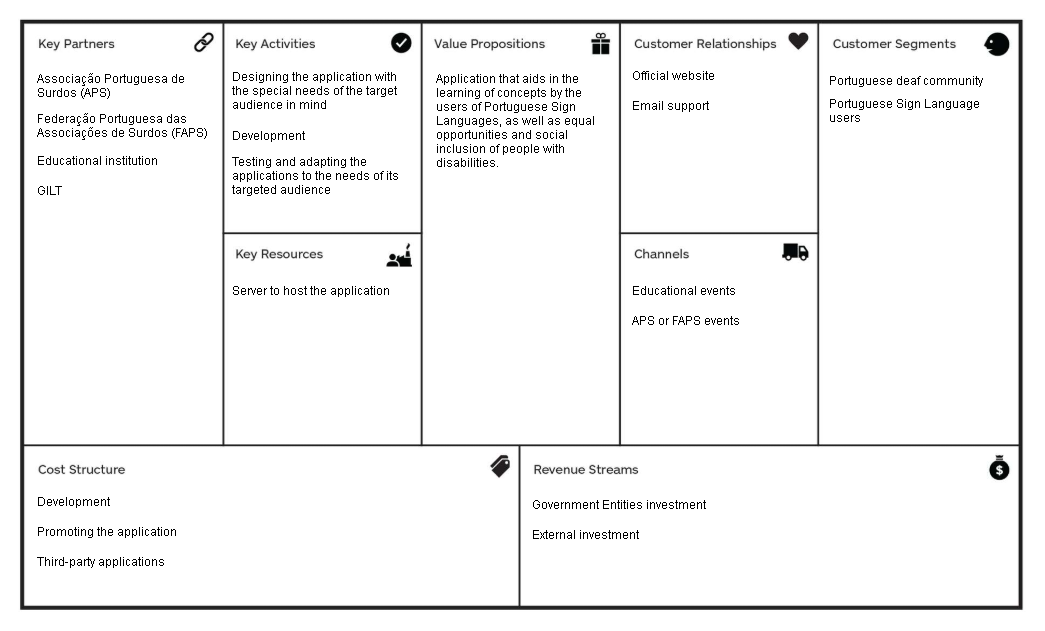
\includegraphics[width=\textwidth,keepaspectratio]{ch3/assets/CANVAS.png}
\caption[Canvas Model]{Canvas Model}
\label{fig:CANVAS}
\end{figure}

The solution developed has two customer segments, which are the Portuguese deaf community and the Portuguese Sign Language users.

As for the product to be provided to this customers, it will be an application that aids in the learning of concepts by the users of Portuguese Sign Language.
By doing so it will help to provide equal opportunities and social inclusion of people with disabilities.

To reach the target audience it should be presented in educational events and in events of the Portuguese Deaf Association or the Portuguese Federation of Deaf Associations.

The customers can expect to find this solution on a website, with all the information needed and the possibility to clarify any doubts through the email support.

In regards to the revenue this solution can get, it will have its origins in the investment made by External companies or Government Entities.

When it comes to the resources required, the most important is the server to host the application to ensure maximum availability.

To increase the chances for the solution to succeed, it is priority to design and develop the application with the special needs of the target audience in mind.
As well as testing and adapting the solution if/when their needs fail to be met.

This solution is in the best interest of education institutions, the Portuguese Deaf Association, the Portuguese Federation of Deaf Associations and GILT so they will be the key partners.

Finally, the costs will have their origin in the development and promotion of the application as well as any third-party application required to be used while escalating the solution.

\section{Analytic Hierarchy Process (AHP)}

The \gls{AHP} was introduced by Saaty\cite{saaty1987analytic} and is an efficient tool to use in the process of complex decision making.
It allows to define priorities using qualitative and quantitative criteria to help reduce complex decisions to a series of paired comparisons.
Using this method will also reduce the bias in process of choice.

\subsection{Stage 1 - Creating the hierarchical decision tree}

This stage consists in creating the hierarchical decision tree where the criteria and viable alternatives are defined.
In regard to the problem, it goal is to determine which natural language processing tools will provide the most value for the project.
The created hierarchical decision tree is presented in the Figure~\ref{fig:AHP}.

\begin{figure}[H]
\centering
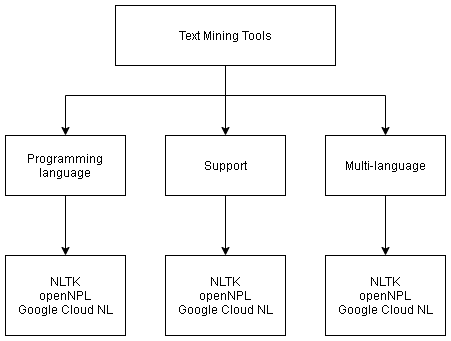
\includegraphics[scale=0.6]{ch3/assets/AHP.png}
\caption[Hierarchical Decision Tree]{Hierarchical Decision Tree}
\label{fig:AHP}
\end{figure}

As observed in the image above, the items of the first layer, corresponding to the primary objectives, had the following criteria behind their selection:
\begin{itemize}
    \item \textbf{Programming language} - The programming language required to be used by the natural language processing tool when developing a solution (e.g. Python, Java, C, JavaScript, etc.).
    \item \textbf{Support} - The number and quality of reliable sources of information about each tool (e.g. Books, Documentation, Forums, etc.).
    \item \textbf{Multi-language} - The compatibility of processing texts and performing tasks using natural languages other than English, with special focus in Portuguese.
\end{itemize}

The presented alternatives in the Figure~\ref{fig:AHP} are the selected natural language processing tools.

NLTK was chosen because it represents a tool that already as a lot of trained models that can be easily used for developing a solution.
The fact that  it's a library for Python, is also important since its the preferred programming language.
Also, as mentioned in Chapter~\ref{chap:Chapter2}, the book available for this tool, allows for a first time user to be able to learn quickly.
Furthermore, after a quick web search its easy to find examples of implementation of text mining approaches using this library.

OpenNLP was chosen because, unlike NLTK, it represents a tool that is meant to be train by the user according to the project needs.
Being a Java library has some relevance since its the second preferred programming language.
The available documentation, that is maintained by the developing community, is not as good as NLTK but it's still easy to follow.

Google Cloud NLP was chosen because, unlike the two upper mentioned, it represents a tool that is not open source and therefore presents payed solutions that may be more efficient.
It can be used with multiple programming languages such as, Python, PHP, Java, Go, etc.
One important aspect of this tools, like other Google services, is the extensive and easy to follow documentation with code snippets that are able to be run in their services to have a better understanding them.

There are countless others tools that are able to perform natural language processing, this were the selected ones since they were heavily recommended and can represent a good portion of them.

The tools here mentioned are described in more detail in Chapter~\ref{chap:Chapter2}.

\subsection{Stage 2 - Alternative and criteria comparison}

This stage consists in defining the priorities between the elements of each hierarchical level.
This is created using the Fundamental scale created by Saaty\cite{saaty1987analytic} that is shown in the Table~\ref{tab:scale}.

\begin{table}[H]
\caption{Fundamental scale \cite{saaty1987analytic}.}
\label{tab:scale}
\centering
\begin{tabular}{|m{4cm}|m{4cm}|m{4cm}|}
\hline
\tabhead{Intensity of importance on an absolute scale} & \tabhead{Definition} & \tabhead{Explanation} \\
\hline
1 & Equal importance & Two activities contribute equally to the objective\\
\hline
3 & Moderate importance of one over another & Experience and judgment strongly favor one activity over another\\
\hline
5 & Essential or strong importance & Experience and judgment strongly favor one activity over another\\
\hline
7 & Very strong importance & An activity is strongly favored and its dominance demonstrated in practice\\
\hline
9 & Extreme importance & The evidence favoring one activity over another is of the highest possible order of affirmation \\
\hline
2,4,6,8 & Intermediate values between two adjacent judgments & When compromise is needed \\
\hline
\end{tabular}
\end{table}

Each comparison between two criterion was defined using the values from the table above, after pondering their relative importance.
The Table~\ref{tab:criteria}, was created to present the result of the comparisons made in regards to the criteria of the decision tree.

\begin{table}[H]
\caption{Comparison Criteria.}
\label{tab:criteria}
\centering
\begin{tabular}{|m{4cm}|m{3cm}|m{3cm}|m{3cm}|}
\hline
\tabhead{Criteria} & \tabhead{Programming language} & \tabhead{Support} & \tabhead{Multi-language} \\
\hline
Programming language & 1 & 1/3 & 1/2 \\
\hline
Support & 3 & 1 & 3 \\
\hline
Multi-language & 2 & 1/3 & 1 \\
\hline
Sum & 6 & 5/3 & 9/2 \\
\hline
\end{tabular}
\end{table}

With the information in the table above it is possible to assess that the criterion "Support" is of moderate importance (3) in comparison with the "Programming language" criterion, and it is of moderate importance (3) when compared to "Multi-language".
Also the criterion "Multi-language" is of slightly more importance (2) when compared to the "Programming language" criterion.

\subsection{Stage 3 - Relative priority of each criterion}

This stage consists in obtaining the normalized criteria values and its relative priorities.
To accomplish this, each value is divided by the sum of its respective column as shown in the Table~\ref{tab:normalization}.

\begin{table}[H]
\caption{Comparison Criteria Normalized.}
\label{tab:normalization}
\centering
\begin{tabular}{|m{4cm}|m{3cm}|m{3cm}|m{3cm}|}
\hline
\tabhead{Criteria} & \tabhead{Programming language} & \tabhead{Support} & \tabhead{Multi-language} \\
\hline
Programming language & 1/6 & 1/5 & 1/9 \\
\hline
Support & 3/6 & 3/5 & 2/3 \\
\hline
Multi-language & 2/6 & 1/5 & 2/9 \\
\hline
\end{tabular}
\end{table}

Having normalized the criteria values, the next step is to calculate the priority order of each criterion.
To accomplish this the arithmetic mean is used in each normalized criterion values previously obtained, as presented in Table~\ref{tab:relativePriority}.

\begin{table}[H]
\caption{Relative priority.}
\label{tab:relativePriority}
\centering
\begin{tabular}{|m{4cm}|m{4cm}|}
\hline
\tabhead{Criteria} & \tabhead{Relative priority} \\
\hline
Programming language & 0.159 \\
\hline
Support & 0.589 \\
\hline
Multi-language & 0.252 \\
\hline
\end{tabular}
\end{table}

With the values from the table above it's possible to conclude that the principal criterion for choosing one of the alternatives is "Support", followed by "Multi-language" and lastly "Programming language".

\subsection{Stage 4 - Consistency evaluation of relative priorities}

This stage consists in calculating the \gls{CR} to assess the consistency of the priorities used in Table~\ref{tab:criteria}.

To calculate the \gls{CR}, the \gls{CI} and the \gls{RI} are used as shown in the following equation:

\begin{equation}
    CR = \frac{CI}{RI}
\end{equation}

It is possible to calculate the \gls{CI} using the Equation~\ref{eqn:CI}.

\begin{equation}
    \label{eqn:CI}
    CI = \frac{\lambda_{max}-n}{n-1}
\end{equation}

In the above equation, $n$ is the number of criteria and $\lambda_{max}$ is the largest eigenvalue of the matrix.

\begin{gather}
    \label{eqn:preLambda}
    \begin{bmatrix}
        1 & 1/3 & 1/2 \\
        3 & 1 & 3 \\
        2 & 1/3 & 1
    \end{bmatrix}
    *
    \begin{bmatrix}
      0.159 \\
      0.589 \\
      0.252
    \end{bmatrix}
      =
    \begin{bmatrix}
      0.481 \\
      1.822 \\
      0.766
    \end{bmatrix}
\end{gather}


\begin{gather}
    \label{eqn:lambdaMax}
    \lambda_{max} =
    \frac{\frac{0.481}{0.159} + \frac{1.822}{0.589} + \frac{0.766}{0.252}}{3}
    = 3.05
\end{gather}

The $\lambda_{max}$ was obtained in the Equation~\ref{eqn:lambdaMax} by calculating the mean of the resulting values from the Equation~\ref{eqn:preLambda} that multiplies the criteria comparison matrix by its priority vector.

The next step is to calculate the \gls{CI} using the following equation:

\begin{equation}
    CI = \frac{3.05-3}{3-1} = 0.025
\end{equation}

The \gls{RI} can be obtained in the index table provided by Saaty\cite{saaty1987analytic}, were a part of it is presented in Table~\ref{tab:index}.

\begin{table}[H]
\caption{Index Table \cite{saaty1987analytic}.}
\label{tab:index}
\centering
\begin{tabular}{|m{1cm}|m{1cm}|m{1cm}|m{1cm}|m{1cm}|m{1cm}|}
\hline
\tabhead{N} & \tabhead{1} & \tabhead{2} & \tabhead{3} & \tabhead{4} & \tabhead{5} \\
\hline
RI & 0 & 0 & 0.58 & 0.90 & 1.12 \\
\hline
\end{tabular}
\end{table}

The \gls{RI} used will be 0.58 since the $n$, as previously is 3.

Having the \gls{CI} and the \gls{RI} values, it was possible to calculate the \gls{CR} as shown in the following equation:

\begin{equation}
    CR = \frac{0.025}{0.58} = 0.043
\end{equation}

Since the obtained value 0.043 is less than 0.1 it is possible to conclude that the values attributed to the properties are consistent.

\subsection{Stage 5 - Construction of the parity comparison matrix for each criterion}

This stage consists in creating a parity comparison matrix for each of the alternatives presented in the hierarchical decision tree, these are the natural language processing tools.
The relative priorities were calculated as shown previously in Stage 3.

\begin{table}[H]
\caption{Programming Language Parity Comparison Matrix.}
\label{tab:progLangPC}
\centering
\begin{tabular}{|m{3cm}|m{3cm}|m{3cm}|m{3cm}|}
\hline
\tabhead{Programming Language} & \tabhead{NLTK} & \tabhead{openNLP} & \tabhead{Google Cloud NL} \\
\hline
NLTK & 1 & 5 & 1/2 \\
\hline
openNLP & 1/5 & 1 & 1/5 \\
\hline
Google Cloud NL & 2 & 5 & 1 \\
\hline
Sum & 16/5 & 11 & 17/10 \\
\hline
\end{tabular}
\end{table}

\begin{table}[H]
\caption{Programming Language Relative Priority.}
\label{tab:progLangPCRP}
\centering
\begin{tabular}{|m{3cm}|m{3cm}|}
\hline
\tabhead{Programming Language} & \tabhead{Relative Priority} \\
\hline
NLTK & 0.354 \\
\hline
openNLP & 0.090 \\
\hline
Google Cloud NL & 0.598 \\
\hline
\end{tabular}
\end{table}

\begin{table}[H]
\caption{Support Parity Comparison Matrix.}
\label{tab:supportPC}
\centering
\begin{tabular}{|m{3cm}|m{3cm}|m{3cm}|m{3cm}|}
\hline
\tabhead{Support} & \tabhead{NLTK} & \tabhead{openNLP} & \tabhead{Google Cloud NL} \\
\hline
NLTK & 1 & 3 & 5 \\
\hline
openNLP & 1/3 & 1 & 3 \\
\hline
Google Cloud NL & 1/5 & 1/3 & 1 \\
\hline
Sum & 23/15 & 13/3 & 9 \\
\hline
\end{tabular}
\end{table}

\begin{table}[H]
\caption{Support Relative Priority.}
\label{tab:supportPCRP}
\centering
\begin{tabular}{|m{3cm}|m{3cm}|}
\hline
\tabhead{Support} & \tabhead{Relative Priority} \\
\hline
NLTK & 0.633 \\
\hline
openNLP & 0.260 \\
\hline
Google Cloud NL & 0.106 \\
\hline
\end{tabular}
\end{table}

\begin{table}[H]
\caption{Multi-language Comparison Matrix.}
\label{tab:multiLangPC}
\centering
\begin{tabular}{|m{3cm}|m{3cm}|m{3cm}|m{3cm}|}
\hline
\tabhead{Multi-language} & \tabhead{NLTK} & \tabhead{openNLP} & \tabhead{Google Cloud NL} \\
\hline
NLTK & 1 & 4 & 1/2 \\
\hline
openNLP & 1/4 & 1 & 1/5 \\
\hline
Google Cloud NL & 2 & 5 & 1 \\
\hline
Sum & 13/4 & 10 & 17/10 \\
\hline
\end{tabular}
\end{table}

\begin{table}[H]
\caption{Multi-language Relative Priority.}
\label{tab:multiLangPCRP}
\centering
\begin{tabular}{|m{3cm}|m{3cm}|}
\hline
\tabhead{Multi-language} & \tabhead{Relative Priority} \\
\hline
NLTK & 0.334 \\
\hline
openNLP & 0.098 \\
\hline
Google Cloud NL & 0.568  \\
\hline
\end{tabular}
\end{table}

To conclude this stage, the hierarchical decision tree was recreated with the all the calculated values, as shown in the Figure~\ref{fig:AHPWeighted}.

\begin{figure}[H]
\centering
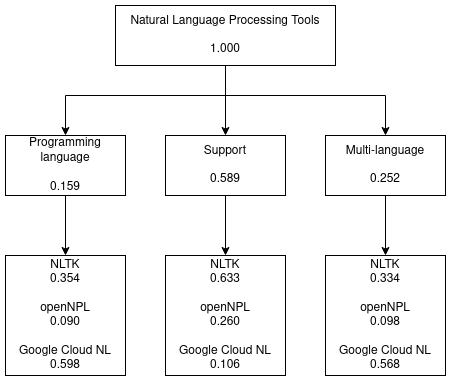
\includegraphics[scale=0.6]{ch3/assets/AHP_weighted.png}
\caption[Hierarchical decision tree with criteria parity comparison]{Hierarchical decision tree with criteria parity comparison}
\label{fig:AHPWeighted}
\end{figure}

\subsection{Stage 6 - Obtain the composite property for alternatives}

This stage consists in obtaining the composite property for the alternatives, to accomplish this, the matrix composed by each criterion relative priority is multiplied by the criteria weight as shown in the following equation:

\begin{gather}
    \begin{bmatrix}
        0.354 & 0.633 & 0.334 \\
        0.090 & 0.260 & 0.098 \\
        0.598 & 0.106 & 0.568
    \end{bmatrix}
    *
    \begin{bmatrix}
      0.159 \\
      0.589 \\
      0.252
    \end{bmatrix}
      =
    \begin{bmatrix}
      \textbf{0.513} \\
      0.192 \\
      0.301
    \end{bmatrix}
\end{gather}

\subsection{Stage 7 - Choice of alternative}

This stage consists in analyzing the obtained values and determine which is the best alternative.
Looking at the obtained values, with the criteria selected and its calculated importance in mind, it is safe to affirm that the best option is NLTK since it obtained the highest valued (0.513).
With the results from this process, the solution to be developed in this project will use NLTK as its natural language processing tool.

% Chapter 4

\chapter{Analysis and Design} % Main chapter title
\label{chap:Chapter4} 

In this chapter is possible to find the design progression and the reasoning behind it.wwww

The first step to design a possible solution was to create a high-level view of the main functionalities the application should have.

\begin{figure}[H]
\centering
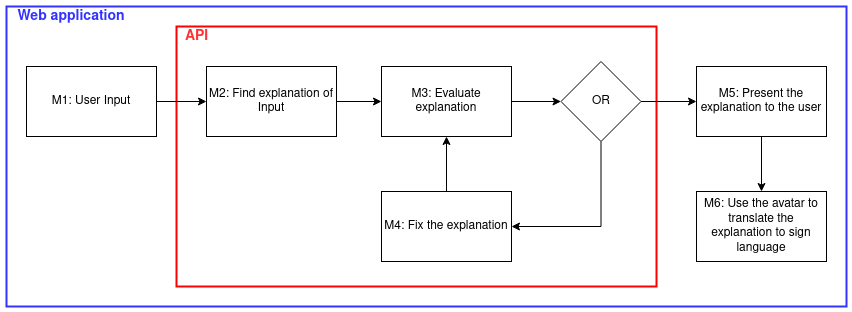
\includegraphics[scale=0.5]{ch4/assets/diagram1_2.png}
\caption[High-Level Approach]{High-Level Approach}
\label{fig:Diagram1}
\end{figure}

In the Figure~\ref{fig:Diagram1} is shown the main build blocks of the web application to be developed.
The input received in M1 is send to the \gls{API} that generates an explanation in M2, which is validated in M3.
From there the explanation might be sent back to the application and shown to the user in M5  or if does not meet all the creteria defined in M3 it will be fixed in M4 and reevaluated.
After presenting the explanation to the user, the application will also be capable of send the text to an already existing \gls{API} that is capable of translate plain text to \gls{PSL} using a avatar in M6.

To help better understand the created design, a more detailed view, is presented below, that describes each of the build blocks and how will they achieve the tasks previously mentioned.

\begin{figure}[H]
\centering
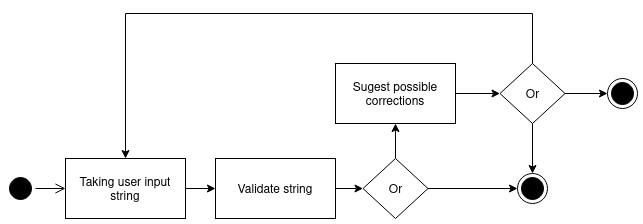
\includegraphics[scale=0.5]{ch4/assets/M1.png}
\caption[User Input Module]{M1: User Input}
\label{fig:M1}
\end{figure}

As shown in the Figure~\ref{fig:M1} the M1 was design to receive a input string from the user.
This string is validated in order to dected common mistakes, such as typos, and when an mistake is detected the application suggests possible corrections.
The user is then capable of accepting the suggestion given, make a manual correction or procede without changing the input string.

\begin{figure}[H]
\centering
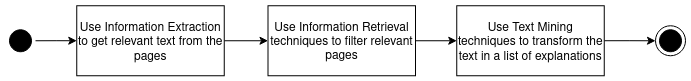
\includegraphics[scale=0.5]{ch4/assets/M2.png}
\caption[Find Explanation Module]{M2: Find Explanation}
\label{fig:M2}
\end{figure}

The Figure~\ref{fig:M2} shows the process of finding an explanation based on the received string.
A web crawler would be use to find all the pages connected to the one \dots

\begin{figure}[H]
\centering
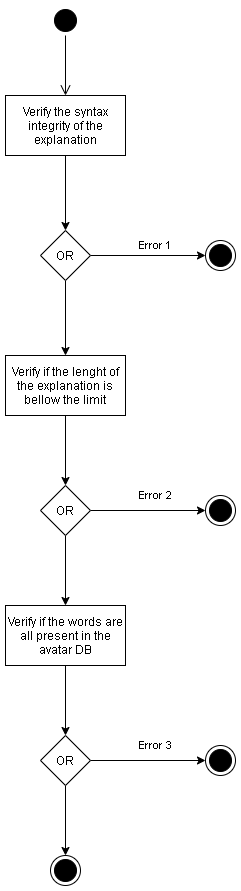
\includegraphics[scale=0.5]{ch4/assets/M3.png}
\caption[Evaluate Explanation Module]{M3: Evaluta Explanation}
\label{fig:M3}
\end{figure}

In Figure~\ref{fig:M3}

\begin{figure}[H]
\centering
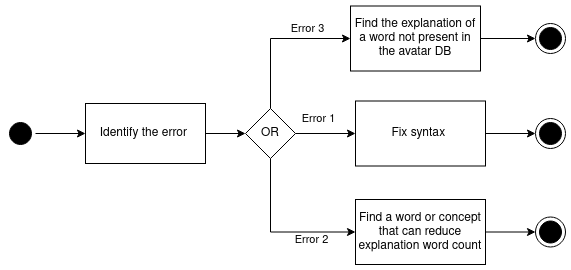
\includegraphics[width=\textwidth,keepaspectratio]{ch4/assets/M4.png}
\caption[Fix Explanation Module]{M4: Fix Explanation}
\label{fig:M4}
\end{figure}

As it can be seen in Figure~\ref{fig:M4}

\begin{figure}[H]
\centering
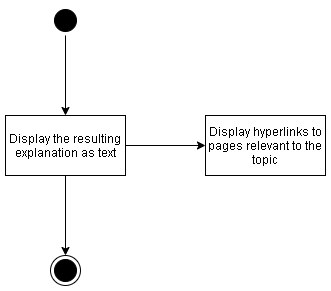
\includegraphics[scale=0.5]{ch4/assets/M5.png}
\caption[Present Explanation Module]{M5: Present Explanation}
\label{fig:M5}
\end{figure}

Figure~\ref{fig:M5}

\begin{figure}[H]
\centering
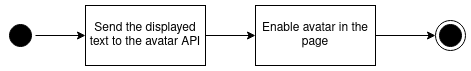
\includegraphics[scale=0.5]{ch4/assets/M6.png}
\caption[Avatar Module]{M6: Avatar}
\label{fig:M6}
\end{figure}

Figure~\ref{fig:M6}


With the complete design of the application in mind a simpler and easier to implement approach was design, also known as a \gls{MVP}.

\begin{figure}[H]
\centering
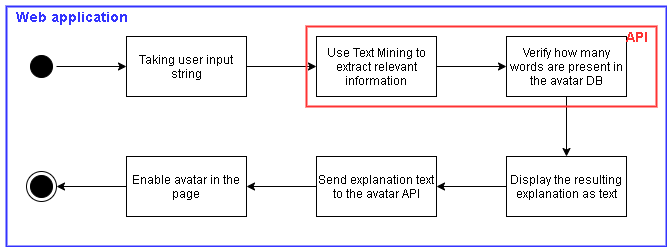
\includegraphics[width=\textwidth,keepaspectratio]{ch4/assets/mvp_2.png}
\caption[Minimun Value Product]{Minimun Value Product}
\label{fig:mvp}
\end{figure}

Figure~\ref{fig:mvp}
% Chapter 5

\chapter{Implementation} % Main chapter title
\label{chap:Chapter5}

\section{LGP Readability Formula}

For a regular language, there are metrics, like the readability score, that can be used to classify each expression in order to sort them accordingly.
This score indicates how easily a reader would comprehend the text that he's reading.

There are multiple formulas that could be used for calculating this score in Portuguese, as shown in Table. %TODO REF.
However, there is none for the LGP.

When looking at the readability formulas for Portuguese, it is easy to notice that, all of them take in consideration the same variables, which are common in every written text: characters, complex words, syllables, words and sentences.

After analyzing the LGP signs, with the goal of creating a new readability calculation formula, all the shared variables where identified:

\begin{itemize}
    \item Hand configurations (CF) - The hand shape in a particular moment.
    \item Moments (MT) - The position of the hand in relation to the body.
    \item Hands (HS) - Both hands or only the dominant hand.
    \item Facial expressions (FE) - Motion or position of the face muscles.
\end{itemize}

Using those variables the following formula was created:

\begin{equation}
(0.7 \times CF + 0.3 \times MT + 1 \times FE) \times (0.5 \times HS)
\label{wordScore}
\end{equation}

This formula allows to calculate the readability score of a word in LGP.
In order to calculate the score of an entire sentence, the sum of the scores of each word were divided by the number of words in the sentence, creating the following formula:

\begin{equation}
    \frac{(0.7 \times CF + 0.3 \times MT + 1 \times FE) \times (0.5 \times HS)}{WO}
\label{sentecneScore}
\end{equation}

\dots


% Chapter 6

\chapter{Evaluation} % Main chapter title
\label{chap:Chapter6}

During the development of a solution it is necessary to evaluate its quality as well as if it resolves the problems for what it was created to.
This chapter aims to assess the developed solution using tests and experiments and analyzing their outcome.

\section{Evaluation metrics}

In order to evaluate the developed solution for the problem exposed in the Section 1.2 there needs to be test the following features:

\begin{itemize}
    \item The ability for a user to understand a concept based on a generated explanation.
    \item The usability of the website for the deaf community.
    \item The performance of the used text mining algorithms.
    \item The technical quality of the solution.
\end{itemize}

\section{Hypotheses}

A hypothesis was defined in order for the project to be able to help the creation of \gls{LGP} content, and by doing so promoting the inclusion and equality of opportunities for the deaf community.
This hypothesis consists in verifying if it is possible to utilize text mining algorithms to generate the explanation of a given word or expression for users of \gls{LGP}.

After it has been defined, the hypothesis will be tested using evaluating methodologies in order to assess its validation.

\section{Methodologies}

The technical quality of the solution is measure using tests, namely integration tests, functional tests and system tests.
Has the development gets to a state where those tests are reliable, they will be executed using specific tools  namely unitary and of integration, which are run using specific tools.

The usability of the website and the ability to understand a concept based on the generated explanation will be evaluated using surveys.
For the usability the surveys to be used will be the SUS (System Usability Scale).
The criteria for this survey are the following:

\begin{itemize}
    \item Effectiveness - Evaluates if the website users were able to achieve their goals.
    \item Efficiency - Evaluates the effort and resources needed for the users to achieve their goals.
    \item Satisfaction - Evaluates the satisfaction of the users experience.
\end{itemize}

The utilization of text mining algorithms requires specific metrics to evaluate its performance.
This metrics are:

\begin{itemize}
    \item Accuracy - It is the fraction of the correct predictions made by the model.
    It can be calculated using the following formula:

    \begin{equation}
    Accuracy = \frac{True Positives + True Negatives}{Total number of predictions}
    \label{eqn:Accuracy}
    \end{equation}

    \item Precision - It is the fraction of positive identification among all the identifications made by the model.
    It can be calculated using the following formula:

    \begin{equation}
    Precision = \frac{True Positives}{True Positives + False Positives}
    \label{eqn:Precision}
    \end{equation}

    \item Recall - It is the fraction of positive identification among all the possible identification to be made.
    It can be calculated using the following formula:

    \begin{equation}
    Recall = \frac{True Positives}{True Positives + False Negatives}
    \label{eqn:Recall}
    \end{equation}

    \item F-measure - It is the harmonic mean between Recall and Precision, in order to give a better perception of both in a single value.
    It can be calculated using the following formula:

    \begin{equation}
    F-measure = \frac{2*{Precision}*{Recall}}{Precision + Recall}
    \label{eqn:F-measure}
    \end{equation}

\end{itemize}

% Chapter 7

\chapter{Conclusion} % Main chapter title
\label{chap:Chapter7} 


%----------------------------------------------------------------------------------------
%	BIBLIOGRAPHY
%----------------------------------------------------------------------------------------

\printbibliography[heading=bibintoc]

%----------------------------------------------------------------------------------------
%	THESIS CONTENT - APPENDICES
%----------------------------------------------------------------------------------------

\appendix % Cue to tell LaTeX that the following "chapters" are Appendices

% Include the appendices of the thesis as separate files from the Appendices folder
% Uncomment the lines as you write the Appendices

%% Appendix A

\chapter{Application Survey} % Main appendix title

\label{AppendixA} % For referencing this appendix elsewhere, use \ref{AppendixA}

\begin{figure}[H]
    \centering
    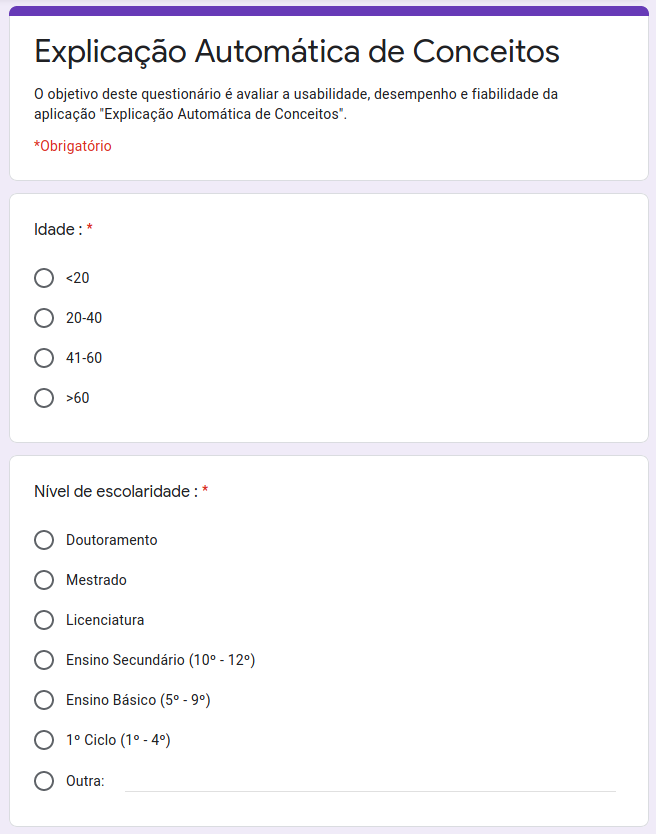
\includegraphics[scale=0.7]{appendices/assets/survey1.png}
    \label{fig:survey1}
\end{figure}

\begin{figure}[H]
    \centering
    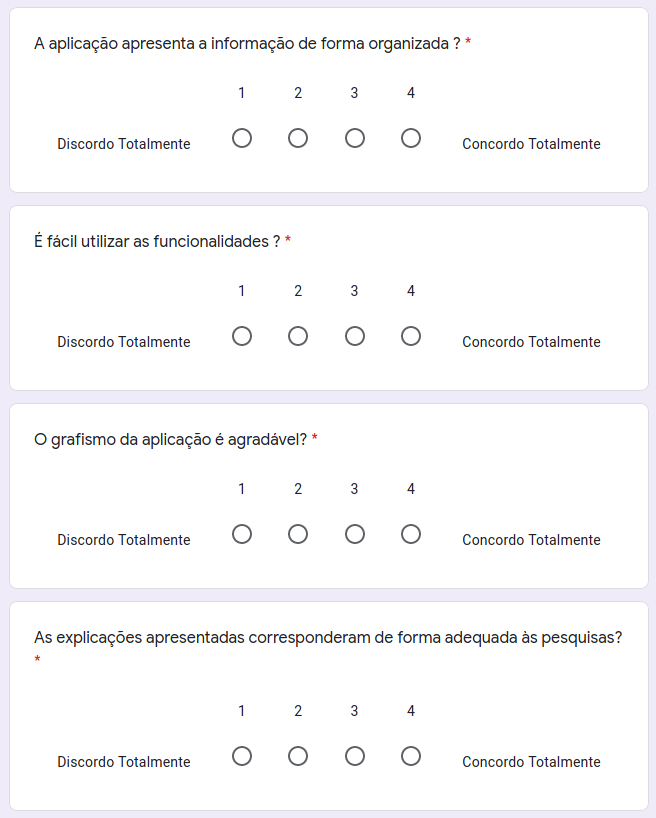
\includegraphics[scale=0.7]{appendices/assets/survey2.png}
    \label{fig:survey1}
\end{figure}

\begin{figure}[H]
    \centering
    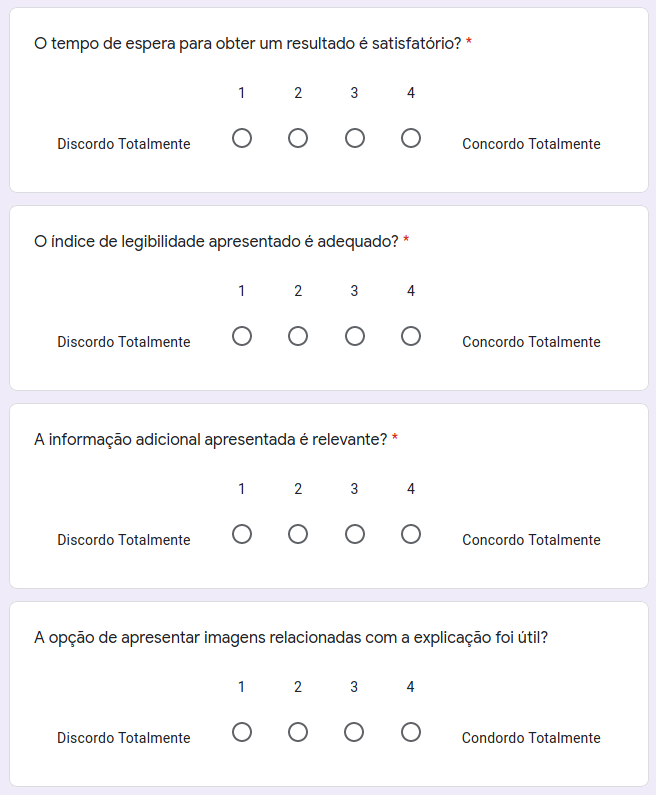
\includegraphics[scale=0.7]{appendices/assets/survey3.png}
    \label{fig:survey1}
\end{figure}

\begin{figure}[H]
    \centering
    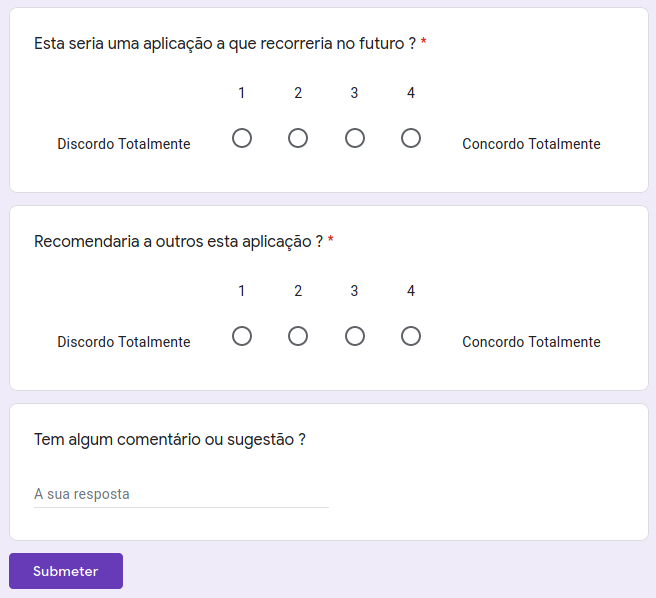
\includegraphics[scale=0.7]{appendices/assets/survey4.png}
    \label{fig:survey1}
\end{figure}



%\input{appendices/appendixB}
%\input{appendices/appendixC}

%----------------------------------------------------------------------------------------

\end{document}
